\documentclass[tikz,border=2pt]{standalone}
\usepackage{amsmath}
\usepackage{pgfplots}
\pgfplotsset{compat=1.18}
\usetikzlibrary{arrows.meta}
\begin{document}
% matrix(1:6 values, nrow = 3) fills column by column; byrow = TRUE fills row by row.
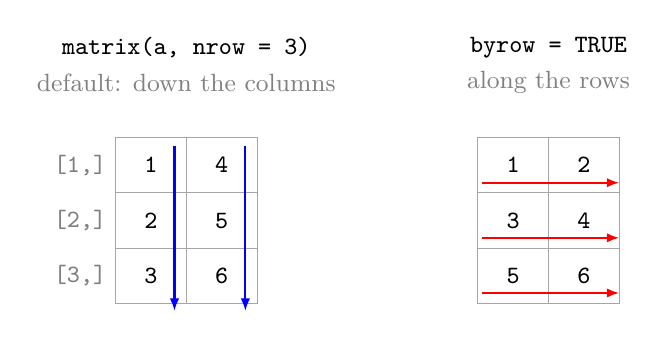
\begin{tikzpicture}[font=\small, >={Latex[length=1.6mm]},
  cell/.style={draw, gray!70, minimum width=9mm, minimum height=7mm, inner sep=0pt, font=\small\ttfamily, text=black}]
  % left: column-wise
  \node[font=\small\ttfamily] at (1.35,3.0) {matrix(a, nrow = 3)};
  \node[gray] at (1.35,2.55) {default: down the columns};
  \foreach \c in {1,2} \foreach \r in {1,2,3} {
    \pgfmathtruncatemacro{\v}{\r+3*(\c-1)}
    \node[cell] at (0.9*\c,2.2-0.7*\r) {\v};
  }
  \foreach \c in {1,2} \draw[->, thick, blue] (0.9*\c+0.3,1.75) -- (0.9*\c+0.3,-0.35);
  % right: row-wise
  \begin{scope}[xshift=4.6cm]
    \node[font=\small\ttfamily] at (1.35,3.0) {byrow = TRUE};
    \node[gray] at (1.35,2.55) {along the rows};
    \foreach \c in {1,2} \foreach \r in {1,2,3} {
      \pgfmathtruncatemacro{\v}{\c+2*(\r-1)}
      \node[cell] at (0.9*\c,2.2-0.7*\r) {\v};
    }
    \foreach \r in {1,2,3} \draw[->, thick, red] (0.5,2.2-0.7*\r-0.22) -- (2.25,2.2-0.7*\r-0.22);
  \end{scope}
  \node[gray, font=\small\ttfamily] at (0.0,1.5) {[1,]};
  \node[gray, font=\small\ttfamily] at (0.0,0.8) {[2,]};
  \node[gray, font=\small\ttfamily] at (0.0,0.1) {[3,]};
\end{tikzpicture}
\end{document}
